\section*{Feynman rules in QCD}
\label{Feynman}
\begin{figure}[h!]
\hspace{-1cm}
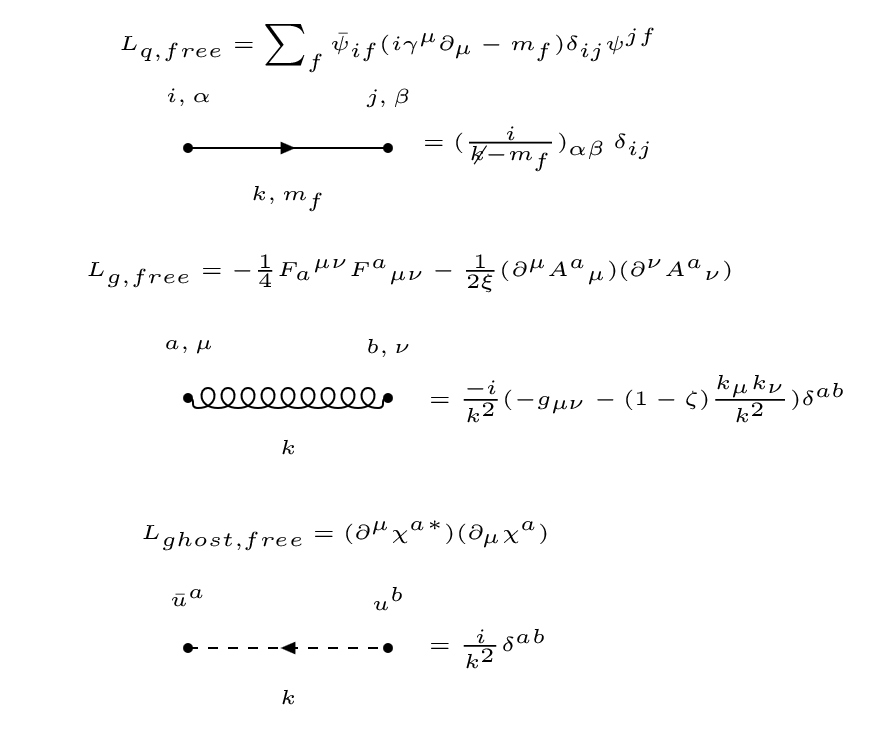
\includegraphics[scale=0.7]{images/Intro/Lfree.png}
\end{figure}

\begin{figure}[h!]
\hspace{-1cm}
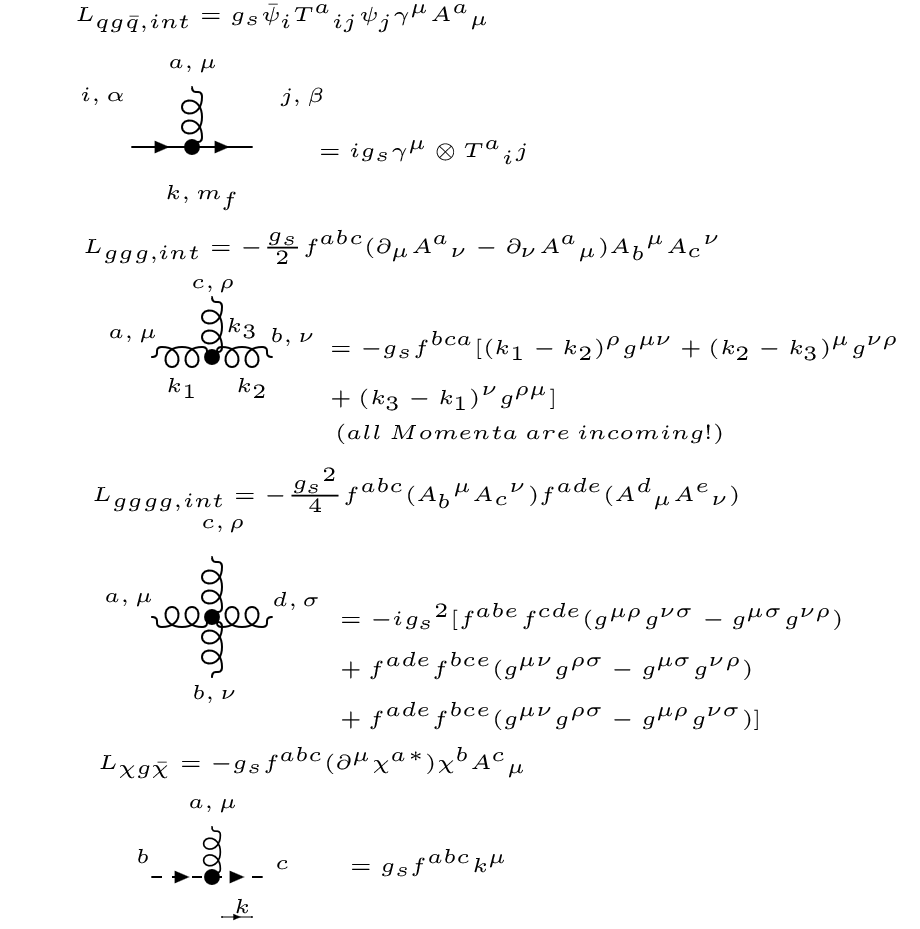
\includegraphics[scale=0.7]{images/Intro/Lint.png}
\end{figure}

\section*{Lorenz transformation of momenta $ {\hat{{p_i}}}^{\mu}, {\hat{{p_k}}}^{\mu} $ and $ {\hat{{Q}}}^{\mu} $}
\begin{equation*}
\begin{split}
&{\hat{{p_i}}}^{\mu}=\alpha{\Lambda^{\mu}}_{\nu} {p_i}^{\nu}= {p_i}^{\mu} p_{i\nu}{p_i}^{\nu} \frac{-y^2 Q^2}{4(p_i\cdot Q)^2(1+\sqrt{1-y}-\frac{y}{2})}
	+{p_i}^{\mu} Q_{\nu}{p_i}^{\nu} \frac{y(1+\sqrt{1-y})}{2(p_i\cdot Q)(1+\sqrt{1-y}-\frac{y}{2})}\\
&+{Q}^{\mu} p_{i\nu}{p_i}^{\nu} \frac{(y^2 -y-y\sqrt{1-y})}{2(p_i\cdot Q)(1+\sqrt{1-y}-\frac{y}{2})}+\sqrt{1-y} {\eta^{\mu}}_{\nu}{p_i}^{\nu}\\
\end{split}
\end{equation*}

\begin{equation*}
\begin{split}
&{\hat{{p_i}}}^{\mu}={p_i}^{\mu} (Q\cdot p_i) \frac{y(1+\sqrt{1-y})}{2(p_i\cdot Q)(1+\sqrt{1-y}-\frac{y}{2})}+\sqrt{1-y} {p_i}^{\mu}\\
&={p_i}^{\mu} [ \frac{y(1+\sqrt{1-y})}{(2+2\sqrt{1-y}-y)}+\sqrt{1-y}]={p_i}^{\mu}
    \end{split}
\end{equation*}

\begin{equation}
	\begin{aligned}
		\fbox{$  {\hat{{p_i}}}^{\mu}=\alpha{\Lambda^{\mu}}_{\nu} {p_i}^{\nu}= {p_i}^{\mu}$}
    \end{aligned}
\end{equation}


\begin{equation*}
	\begin{aligned}
	{\hat{{p_k}}}^{\mu}=\alpha{\Lambda^{\mu}}_{\nu} {p_k}^{\nu}= {p_i}^{\mu}[  \frac{-y^2 Q^2 (p_{i}\cdot {p_k})}{4(p_i\cdot Q)^2(1+\sqrt{1-y}-\frac{y}{2})}+ \frac{y(1+\sqrt{1-y})(Q \cdot {p_k})}{2(p_i\cdot Q)(1+\sqrt{1-y}-\frac{y}{2})}]\\
	+{Q}^{\mu} [ \frac{(y^2 -y-y\sqrt{1-y}) (p_{i}\cdot {p_k})}{2(p_i\cdot Q)(1+\sqrt{1-y}-\frac{y}{2})}]
	+\sqrt{1-y} {p_k}^{\mu}\\
    \end{aligned}
\end{equation*}


\begin{equation*}
	\begin{aligned}
	{\hat{{p_k}}}^{\mu}&=\alpha{\Lambda^{\mu}}_{\nu} {p_k}^{\nu}= {p_i}^{\mu}[  \frac{-y^2 Q^2 (p_{i}\cdot {p_k})}{4(p_i\cdot Q)^2(1+\sqrt{1-y}-\frac{y}{2})}+ \frac{y(1+\sqrt{1-y})(Q \cdot {p_k})}{2(p_i\cdot Q)(1+\sqrt{1-y}-\frac{y}{2})}]\\
	&+{Q}^{\mu} [ \frac{(y^2 -y-y\sqrt{1-y}) (p_{i}\cdot {p_k})}{2(p_i\cdot Q)(1+\sqrt{1-y}-\frac{y}{2})}]+\sqrt{1-y} {p_k}^{\mu}\\	
\text{with}\\
	A_1 &\equiv  \frac{-y^2 Q^2 (p_{i}\cdot {p_k})}{4(p_i\cdot Q)^2(1+\sqrt{1-y}-\frac{y}{2})}+ \frac{y(1+\sqrt{1-y})(Q \cdot {p_k})}{2(p_i\cdot Q)(1+\sqrt{1-y}-\frac{y}{2})}\\
		A_2 &\equiv   \frac{(y^2 -y-y\sqrt{1-y}) (p_{i}\cdot {p_k})}{2(p_i\cdot Q)(1+\sqrt{1-y}-\frac{y}{2})}\:\:\:\:\:\:\:\:\:\:\:\:\:\:\:\:\:\:\:\:\:\:\:\:\:\:\:\:\:\:\:\:\:\:\:\:\:\:\:\:\:\:\:\:\:\:\:\:\:\:\:\:\:\:\\\
    \end{aligned}    
\end{equation*}

\begin{equation}
	\begin{aligned}
		\fbox{$  {\hat{{p_k}}}^{\mu}= A_1 \:{p_i}^{\mu}+A_2\:{Q}^{\mu}+\sqrt{1-y} {p_k}^{\mu} $}
    \end{aligned}
\end{equation}

\begin{equation*}
	\begin{aligned}
	{\hat{{Q}}}^{\mu}&=\alpha{\Lambda^{\mu}}_{\nu} {Q}^{\nu}= {p_i}^{\mu}[  \frac{-y^2 Q^2 (p_{i}\cdot {Q})}{4(p_i\cdot Q)^2(1+\sqrt{1-y}-\frac{y}{2})}+ \frac{y(1+\sqrt{1-y})Q^2}{2(p_i\cdot Q)(1+\sqrt{1-y}-\frac{y}{2})}]\\
	&+{Q}^{\mu} [ \frac{(y^2 -y-y\sqrt{1-y}) (p_{i}\cdot {Q})}{2(p_i\cdot Q)(1+\sqrt{1-y}-\frac{y}{2})}]
	+\sqrt{1-y} {Q}^{\mu}\\
\text{with}\\
	S_1 &\equiv  \frac{Q^2}{2p_i \cdot Q}[\frac{-y^2}{2(1+\sqrt{1-y}-\frac{y}{2})}+ \frac{y(1+\sqrt{1-y})}{(1+\sqrt{1-y}-\frac{y}{2})}]=\frac{Q^2}{2p_i \cdot Q}y\\
		S_2 &\equiv   \frac{(y^2 -y-y\sqrt{1-y})}{2(1+\sqrt{1-y}-\frac{y}{2})}+\sqrt{1-y}=1-y\:\:\:\:\:\:\:\:\:\:\:\:\:\:\:\:\:\:\:\:\:\:\:\:\:\:\:\:\:\:\:\:\:\:\:\:\:\:\:\:\:\:\:\:\:\:\:\:\:\:\:\:\:\:\\\	
    \end{aligned}    
\end{equation*}

\begin{equation}
	\begin{aligned}
		\fbox{$  {\hat{{Q}}}^{\mu}= \frac{Q^2}{2p_i \cdot Q}y \:{p_i}^{\mu}+(1-y)\:{Q}^{\mu} $}
    \end{aligned}
\end{equation}

\section*{The often occurring pre-factor products}

\begin{equation}
	\begin{split}
	&\zeta_1\zeta_1=({\alpha_1}^2 -2y\alpha_1 \beta_1(\frac{Q^2}{2p_i \cdot Q})+y^2{\beta_1}^2(\frac{Q^2}{2p_i \cdot Q})^2)\\
	&\zeta_1\lambda_1=(y\alpha_1\beta_1 -{y^2\beta_1}^2(\frac{Q^2}{2p_i \cdot Q}))\\
	&\zeta_1\zeta_q=(\alpha_1\beta_1-y({\alpha_1}^2+{\beta_1}^2) (\frac{Q^2}{2p_i \cdot Q})+y^2{\alpha_1}{\beta_1}(\frac{Q^2}{2p_i \cdot Q})^2)\\
	&\zeta_1\lambda_q=(y{\alpha_1}^2 -y^2\beta_1\alpha_1(\frac{Q^2}{2p_i \cdot Q}))\\
	&\zeta_q\zeta_q=	({\beta_1}^2 -2y\alpha_1\beta_1 (\frac{Q^2}{2p_i \cdot Q})+ y^2{\alpha_1}^2 (\frac{Q^2}{2p_i \cdot Q})^2) \\
	&\zeta_q\lambda_1=(y{\beta_1}^2 -y^2\alpha_1 \beta_1(\frac{Q^2}{2p_i \cdot Q}))\\
	&\zeta_q\lambda_q=(y\beta_1\alpha_1 -y^2{\alpha_1}^2(\frac{Q^2}{2p_i \cdot Q}))\\
	&\lambda_1\lambda_1=y^2{\beta_1}^2 \:\:\:\:\:\:\:
	\lambda_1\lambda_q=y^2\beta_1\alpha_1\:\:\:\:\:\:\:\:
	\lambda_q\lambda_q=y^2{\alpha_1}^2\\
    \end{split}
\end{equation}

\section*{Common scalar products}

\begin{equation}
	\begin{aligned}	
k_1 \cdot q_i &= (\zeta_1 \lambda_q + \lambda_1 \zeta_q)p_i \cdot Q+\lambda_1 \lambda_q Q^2 -y\alpha_1\beta_1 {n^{2}}_{\bot,1}\\
	&=[(\alpha_1 -y\beta_1(\frac{Q^2}{2p_i \cdot Q}))y\alpha_1+y\beta_1(\beta_1 -\alpha_1 y(\frac{Q^2}{2p_i \cdot Q}))]\:p_i \cdot Q\\
	&\:\:\:\:\:\:\:y^2\beta_1\alpha_1\: Q^2+2y\alpha_1\beta_1\:p_iQ\\
\Rightarrow	k_1 \cdot q_i &=[y{\alpha_1}^2 -y^2\alpha_1\beta_1(\frac{Q^2}{2p_i \cdot Q})+y {\beta_1}^2-y^2\alpha_1\beta_1(\frac{Q^2}{2p_i \cdot Q})]\:p_i\cdot Q\\
	&y^2\beta_1\alpha_1\: Q^2+2y\alpha_1\beta_1\:p_iQ\\	
    \end{aligned}
\end{equation}

\begin{equation}
	\begin{aligned}
		\fbox{$  k_1 \cdot q_i=y({\alpha_1}+\beta_1)^2\:p_i\cdot Q = y\:p_i\cdot Q $}
    \end{aligned}
\end{equation}

\begin{equation}
	\begin{aligned}	
	k_1 \cdot q_k &= (\zeta_1 A_2 + \lambda_1 A_1)p_i \cdot Q+\zeta_1 \sqrt{1-y}\:p_i\cdot p_k + \lambda_1 A_2\:Q^2+ \lambda_1\sqrt{1-y}\:Q\cdot p_k\\
	&+\sqrt{\alpha_1\beta_1y(1-y)} p_k \cdot {n_{\bot,1}}\\	
	&=\lbrace[(\alpha_1 -y\beta_1(\frac{Q^2}{2p_i \cdot Q}))\frac{(y^2 -y-y\sqrt{1-y}) (p_{i}\cdot {p_k})}{2(p_i\cdot Q)(1+\sqrt{1-y}-\frac{y}{2})}]\\&
	+y\beta_1[\frac{-y^2 Q^2 (p_{i}\cdot {p_k})}{4(p_i\cdot Q)^2(1+\sqrt{1-y}-\frac{y}{2})}+ \frac{y(1+\sqrt{1-y})(Q \cdot {p_k})}{2(p_i\cdot Q)(1+\sqrt{1-y}-\frac{y}{2})}]\rbrace\:p_i \cdot Q\\
	&+(\alpha_1 -y\beta_1(\frac{Q^2}{2p_i \cdot Q}))\sqrt{1-y}\:p_i \cdot p_k+y\beta_1\frac{(y^2 -y-y\sqrt{1-y}) (p_{i}\cdot {p_k})}{2(p_i\cdot Q)(1+\sqrt{1-y}-\frac{y}{2})}Q^2\\
	&+y\beta_1\sqrt{1-y} Q\cdot p_k+\sqrt{\alpha_1\beta_1y(1-y)} p_k \cdot {n_{\bot,1}} 
    \end{aligned}
\end{equation}

\begin{equation}
	\begin{aligned}
	k_1 \cdot q_k &= \alpha_1 \frac{(y^2 -y-y\sqrt{1-y}) }{2(1+\sqrt{1-y}-\frac{y}{2})}(p_{i}\cdot {p_k})
	-y\beta_1(\frac{Q^2}{2p_i \cdot Q})\frac{(y^2 -y-y\sqrt{1-y})}{2(1+\sqrt{1-y}-\frac{y}{2})}(p_{i}\cdot {p_k})\\
&+y\beta_1\frac{-y^2 Q^2 }{4(p_i\cdot Q)(1+\sqrt{1-y}-\frac{y}{2})}(p_{i}\cdot {p_k})+ y\beta_1\frac{y(1+\sqrt{1-y})}{2(1+\sqrt{1-y}-\frac{y}{2})}\:Q \cdot p_k\\
	&+\alpha_1 \sqrt{1-y}\:p_i \cdot p_k-y\beta_1(\frac{Q^2}{2p_i \cdot Q})\sqrt{1-y}\:p_i \cdot p_k\\
	&+y\beta_1(\frac{Q^2}{2p_i \cdot Q})\frac{(y^2 -y-y\sqrt{1-y})}{2(1+\sqrt{1-y}-\frac{y}{2})}(p_{i}\cdot {p_k})+y\beta_1\sqrt{1-y}(Q\cdot p_k)\\
	&+\sqrt{\alpha_1\beta_1y(1-y)} p_k \cdot {n_{\bot,1}} 
    \end{aligned}
\end{equation}

\begin{equation}
	\begin{aligned}
	k_1 \cdot q_k &= [\alpha_1 \frac{(y^2 -y-y\sqrt{1-y}) }{2(1+\sqrt{1-y}-\frac{y}{2})}+y\beta_1\frac{-y^2 Q^2 }{4(p_i\cdot Q)(1+\sqrt{1-y}-\frac{y}{2})}+\alpha_1 \sqrt{1-y}\\&-y\beta_1(\frac{Q^2}{2p_i \cdot Q})\sqrt{1-y}]\:p_i \cdot p_k+[y\beta_1\frac{y(1+\sqrt{1-y})}{2(1+\sqrt{1-y}-\frac{y}{2})}+y\beta_1\sqrt{1-y}](Q\cdot p_k)\\
	&+\sqrt{\alpha_1\beta_1y(1-y)} p_k \cdot {n_{\bot,1}} 
    \end{aligned}
\end{equation}

\begin{equation}
	\begin{aligned}
	k_1 \cdot q_k &= \lbrace\alpha_1 [\frac{(y^2 -y-y\sqrt{1-y}) }{2(1+\sqrt{1-y}-\frac{y}{2})}+ \sqrt{1-y}]\\
	&+y\beta_1(\frac{Q^2}{p_i \cdot Q})[\frac{-y^2 }{4(1+\sqrt{1-y}-\frac{y}{2})}-\sqrt{1-y}]\rbrace\:p_i \cdot p_k\\
	&+y\beta_1[\frac{y(1+\sqrt{1-y})}{2(1+\sqrt{1-y}-\frac{y}{2})}+\sqrt{1-y}](Q\cdot p_k)\\
	&+\sqrt{\alpha_1\beta_1y(1-y)} p_k \cdot {n_{\bot,1}} 
    \end{aligned}
\end{equation}

\begin{equation}
	\begin{aligned}
		\fbox{$  k_1 \cdot q_k = [\alpha_1 (1-y)+y\beta_1(\frac{Q^2}{2p_i \cdot Q})]\:p_i \cdot p_k+y\beta_1\:Q\cdot p_k+\sqrt{\alpha_1\beta_1y(1-y)} p_k \cdot {n_{\bot,1}} $}
    \end{aligned}
\end{equation}

\begin{equation}
	\begin{aligned}	
	q_i \cdot q_k &= (\zeta_q A_2 + \lambda_q A_1)p_i \cdot Q+\zeta_q \sqrt{1-y}\:p_i\cdot p_k + \lambda_q A_2\:Q^2+ \lambda_q\sqrt{1-y}\:Q\cdot p_k\\
	&-\sqrt{\alpha_1\beta_1y(1-y)} p_k \cdot {n_{\bot,1}}\\	
	&=\lbrace[(\beta_1 -y\alpha_1(\frac{Q^2}{2p_i \cdot Q}))\frac{(y^2 -y-y\sqrt{1-y}) (p_{i}\cdot {p_k})}{2(p_i\cdot Q)(1+\sqrt{1-y}-\frac{y}{2})}]\\&
	+y\alpha_1[\frac{-y^2 Q^2 (p_{i}\cdot {p_k})}{4(p_i\cdot Q)^2(1+\sqrt{1-y}-\frac{y}{2})}+ \frac{y(1+\sqrt{1-y})(Q \cdot {p_k})}{2(p_i\cdot Q)(1+\sqrt{1-y}-\frac{y}{2})}]\rbrace\:p_i \cdot Q\\
	&+(\beta_1 -y\alpha_1(\frac{Q^2}{2p_i \cdot Q}))\sqrt{1-y}\:p_i \cdot p_k+y\alpha_1\frac{(y^2 -y-y\sqrt{1-y}) (p_{i}\cdot {p_k})}{2(p_i\cdot Q)(1+\sqrt{1-y}-\frac{y}{2})}Q^2\\
	&+y\alpha_1\sqrt{1-y} Q\cdot p_k-\sqrt{\alpha_1\beta_1y(1-y)} p_k \cdot {n_{\bot,1}} 
    \end{aligned}
\end{equation}


\begin{equation}
	\begin{aligned}
	q_i \cdot q_k &= \beta_1 \frac{(y^2 -y-y\sqrt{1-y}) }{2(1+\sqrt{1-y}-\frac{y}{2})}(p_{i}\cdot {p_k})
	-y\alpha_1(\frac{Q^2}{2p_i \cdot Q})\frac{(y^2 -y-y\sqrt{1-y})}{2(1+\sqrt{1-y}-\frac{y}{2})}(p_{i}\cdot {p_k})\\
&+y\alpha_1\frac{-y^2 Q^2 }{4(p_i\cdot Q)(1+\sqrt{1-y}-\frac{y}{2})}(p_{i}\cdot {p_k})+ y\alpha_1\frac{y(1+\sqrt{1-y})}{2(1+\sqrt{1-y}-\frac{y}{2})}\:Q \cdot p_k\\
	&+\beta_1 \sqrt{1-y}\:p_i \cdot p_k-y\alpha_1(\frac{Q^2}{2p_i \cdot Q})\sqrt{1-y}\:p_i \cdot p_k\\
	&+y\alpha_1(\frac{Q^2}{2p_i \cdot Q})\frac{(y^2 -y-y\sqrt{1-y})}{2(1+\sqrt{1-y}-\frac{y}{2})}(p_{i}\cdot {p_k})+y\alpha_1\sqrt{1-y}(Q\cdot p_k)\\
	&-\sqrt{\alpha_1\beta_1y(1-y)} p_k \cdot {n_{\bot,1}} 
    \end{aligned}
\end{equation}

\begin{equation}
	\begin{aligned}
	q_i \cdot q_k &= [\beta_1 \frac{(y^2 -y-y\sqrt{1-y}) }{2(1+\sqrt{1-y}-\frac{y}{2})}+y\alpha_1\frac{-y^2 Q^2 }{4(p_i\cdot Q)(1+\sqrt{1-y}-\frac{y}{2})}+\beta_1 \sqrt{1-y}\\&-y\alpha_1(\frac{Q^2}{2p_i \cdot Q})\sqrt{1-y}]\:p_i \cdot p_k+[y\alpha_1\frac{y(1+\sqrt{1-y})}{2(1+\sqrt{1-y}-\frac{y}{2})}+y\alpha_1\sqrt{1-y}](Q\cdot p_k)\\
	&-\sqrt{\alpha_1\beta_1y(1-y)} p_k \cdot {n_{\bot,1}} 
    \end{aligned}
\end{equation}

\begin{equation}
	\begin{aligned}
	k_1 \cdot q_k &= \lbrace\beta_1 [\frac{(y^2 -y-y\sqrt{1-y}) }{2(1+\sqrt{1-y}-\frac{y}{2})}+ \sqrt{1-y}]\\
	&+y\alpha_1(\frac{Q^2}{p_i \cdot Q})[\frac{-y^2 }{4(1+\sqrt{1-y}-\frac{y}{2})}-\sqrt{1-y}]\rbrace\:p_i \cdot p_k\\
	&+y\alpha_1[\frac{y(1+\sqrt{1-y})}{2(1+\sqrt{1-y}-\frac{y}{2})}+\sqrt{1-y}](Q\cdot p_k)\\
	&-\sqrt{\alpha_1\beta_1y(1-y)} p_k \cdot {n_{\bot,1}} 
    \end{aligned}
\end{equation}

\begin{equation}
	\begin{aligned}
		\fbox{$  q_i \cdot q_k = [\beta_1 (1-y)+y\alpha_1(\frac{Q^2}{2p_i \cdot Q})]\:p_i \cdot p_k+y\alpha_1\:Q\cdot p_k-\sqrt{\alpha_1\beta_1y(1-y)} p_k \cdot {n_{\bot,1}} $}
    \end{aligned}
\end{equation}

\pagebreak